\documentclass[noauthor,nooutcomes,hints,handout]{ximera}

\graphicspath{  
{./}
{./whoAreYou/}
{./drawingWithTheTurtle/}
{./bisectionMethod/}
{./circles/}
{./anglesAndRightTriangles/}
{./lawOfSines/}
{./lawOfCosines/}
{./plotter/}
{./staircases/}
{./pitch/}
{./qualityControl/}
{./symmetry/}
{./nGonBlock/}
}


%% page layout
\usepackage[cm,headings]{fullpage}
\raggedright
\setlength\headheight{13.6pt}


%% fonts
\usepackage{euler}

\usepackage{FiraMono}
\renewcommand\familydefault{\ttdefault} 
\usepackage[defaultmathsizes]{mathastext}
\usepackage[htt]{hyphenat}

\usepackage[T1]{fontenc}
\usepackage[scaled=1]{FiraSans}

%\usepackage{wedn}
\usepackage{pbsi} %% Answer font


\usepackage{cancel} %% strike through in pitch/pitch.tex


%% \usepackage{ulem} %% 
%% \renewcommand{\ULthickness}{2pt}% changes underline thickness

\tikzset{>=stealth}

\usepackage{adjustbox}

\setcounter{titlenumber}{-1}

%% journal style
\makeatletter
\newcommand\journalstyle{%
  \def\activitystyle{activity-chapter}
  \def\maketitle{%
    \addtocounter{titlenumber}{1}%
                {\flushleft\small\sffamily\bfseries\@pretitle\par\vspace{-1.5em}}%
                {\flushleft\LARGE\sffamily\bfseries\thetitlenumber\hspace{1em}\@title \par }%
                {\vskip .6em\noindent\textit\theabstract\setcounter{question}{0}\setcounter{sectiontitlenumber}{0}}%
                    \par\vspace{2em}
                    \phantomsection\addcontentsline{toc}{section}{\thetitlenumber\hspace{1em}\textbf{\@title}}%
                     }}
\makeatother



%% thm like environments
\let\question\relax
\let\endquestion\relax

\newtheoremstyle{QuestionStyle}{\topsep}{\topsep}%%% space between body and thm
		{}                      %%% Thm body font
		{}                              %%% Indent amount (empty = no indent)
		{\bfseries}            %%% Thm head font
		{)}                              %%% Punctuation after thm head
		{ }                           %%% Space after thm head
		{\thmnumber{#2}\thmnote{ \bfseries(#3)}}%%% Thm head spec
\theoremstyle{QuestionStyle}
\newtheorem{question}{}



\let\freeResponse\relax
\let\endfreeResponse\relax

%% \newtheoremstyle{ResponseStyle}{\topsep}{\topsep}%%% space between body and thm
%% 		{\wedn\bfseries}                      %%% Thm body font
%% 		{}                              %%% Indent amount (empty = no indent)
%% 		{\wedn\bfseries}            %%% Thm head font
%% 		{}                              %%% Punctuation after thm head
%% 		{3ex}                           %%% Space after thm head
%% 		{\underline{\underline{\thmname{#1}}}}%%% Thm head spec
%% \theoremstyle{ResponseStyle}

\usepackage[tikz]{mdframed}
\mdfdefinestyle{ResponseStyle}{leftmargin=1cm,linecolor=black,roundcorner=5pt,
, font=\bsifamily,}%font=\wedn\bfseries\upshape,}


\ifhandout
\NewEnviron{freeResponse}{}
\else
%\newtheorem{freeResponse}{Response:}
\newenvironment{freeResponse}{\begin{mdframed}[style=ResponseStyle]}{\end{mdframed}}
\fi



%% attempting to automate outcomes.

%% \newwrite\outcomefile
%%   \immediate\openout\outcomefile=\jobname.oc
%% \renewcommand{\outcome}[1]{\edef\theoutcomes{\theoutcomes #1~}%
%% \immediate\write\outcomefile{\unexpanded{\outcome}{#1}}}

%% \newcommand{\outcomelist}{\begin{itemize}\theoutcomes\end{itemize}}

%% \NewEnviron{listOutcomes}{\small\sffamily
%% After answering the following questions, students should be able to:
%% \begin{itemize}
%% \BODY
%% \end{itemize}
%% }
\usepackage[tikz]{mdframed}
\mdfdefinestyle{OutcomeStyle}{leftmargin=2cm,rightmargin=2cm,linecolor=black,roundcorner=5pt,
, font=\small\sffamily,}%font=\wedn\bfseries\upshape,}
\newenvironment{listOutcomes}{\begin{mdframed}[style=OutcomeStyle]After answering the following questions, students should be able to:\begin{itemize}}{\end{itemize}\end{mdframed}}



%% my commands

\newcommand{\snap}{{\bfseries\itshape\textsf{Snap!}}}
\newcommand{\flavor}{\link[\snap]{https://snap.berkeley.edu/}}
\newcommand{\mooculus}{\textsf{\textbf{MOOC}\textnormal{\textsf{ULUS}}}}


\usepackage{tkz-euclide}
\tikzstyle geometryDiagrams=[rounded corners=.5pt,ultra thick,color=black]
\colorlet{penColor}{black} % Color of a curve in a plot



\ifhandout\newcommand{\mynewpage}{\newpage}\else\newcommand{\mynewpage}{}\fi


\title{Pitch}
\author{Bart Snapp}

\begin{document}
\begin{abstract}
  We think about pitch and slope.
\end{abstract}
\maketitle

\begin{listOutcomes}
\item Give the definitions of pitch and slope.
\item Distinguish between pitch and slope.
\item Solve a problem where slope is given.
\item Deduce the slope in a given context.
\item Use tangent to transform angles into slope and pitch.
\item Critique and dismantle reasonable hypotheses in regard to geometry and arithmetic.
\end{listOutcomes}



The steepness of a roof is called its \textit{slope} or
\textit{pitch}. This is a fraction where the numerator is the
\textit{rise} of the roof and the denominator is the \textit{run}. The
denominator is usually $12$. Moreover, when one talks of ``pitch''
they usually omit the denominator of $12$. Hence
\begin{center}
\fbox{a slope of $\frac{7}{12}$}\quad is the same as\quad \fbox{a pitch of $7$}.
\end{center}
This slope (or pitch) says that the roof goes up $7''$ for every
$12''$. Note there are several other notations for pitch. The one we
are presenting here is not only rather common, it is also
mathematically correct!

\mynewpage


\begin{question}
  Here is a roof that is pointed in the middle:
  \begin{center}
    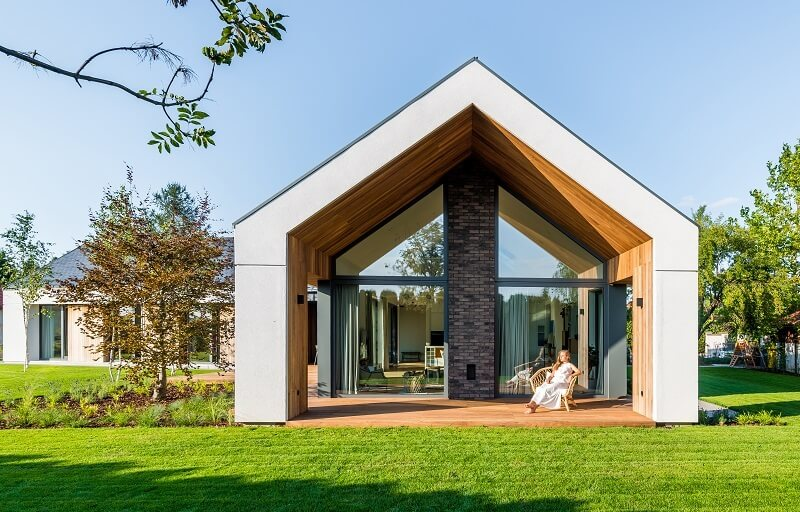
\includegraphics[width=.6\textwidth]{symRoof.jpg}
  \end{center}
Below is a diagram of the roof as seen from the top:
\begin{center}
  \begin{tikzpicture}[x=2cm,y=2cm]
    \draw[ultra thick] (0,0) rectangle (3,2.4);
    %\draw[dashed] (.5,.5) rectangle (4.3,2.5);
    \draw[ultra thick] (0,1.2) -- (3,1.2);
    \draw[decoration={brace,raise=.2cm},decorate,thin] (0,0)--(0,2.4);
    \draw[decoration={brace,raise=.2cm,mirror},decorate,thin] (0,0)--(3,0);
    \node at (-.4,1.2) {$24'$};
    \node at (1.5,-.44) {$30'$};
    \node at (1.5,2.1) {slope of $9/12$};
    \node[above] at (1.5,1.2) {main ridge};
    \node at (1.5,.3) {slope of $9/12$};
  \end{tikzpicture}
\end{center}
Find the area of the roof.  Explain the work in your solution.

\begin{freeResponse}
  If we look at the roof from the side, it looks like:
  \begin{center}
    \begin{tikzpicture}[x=2cm,y=2cm]
    \draw[ultra thick] (0,0) -- (1.2,0)  -- (1.2, .9) -- (0,0) ;
    \draw[decoration={brace,raise=.2cm,mirror},decorate,thin] (0,0)--(1.2,0);
    \draw[decoration={brace,raise=.2cm,mirror},decorate,thin] (1.2,0)--(1.2,.9);
    \node at (.6,-.25) {$12'$};
    \node[anchor=west] at (1.3,.45) {$12'\cdot 9/12$};
    \end{tikzpicture}
    
  \end{center}
    By the Pythagorean theorem, the length of the hypotenuse is
    \[
    \sqrt{12^2+ 9^2} = 15~\text{feet}.
    \]
    Thus, the area of the roof is
    \[
    2\cdot 15\cdot 30 = 900~\text{square feet}.
    \]
\end{freeResponse}
\end{question}
\mynewpage


%% \begin{question}
%%   Here is a roof with different pitches on each side of the main
%%   ridge:
%%   \begin{center}
%%     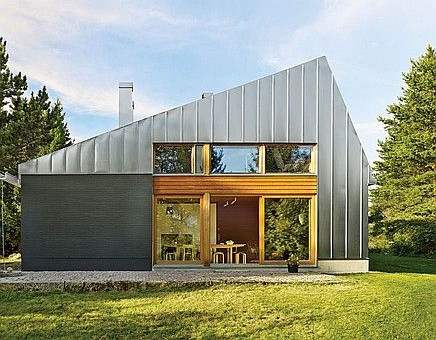
\includegraphics[width=.6\textwidth]{skewRoof.jpg}
%%   \end{center}
%% Below is a diagram of the roof as seen from the top:
%% \begin{center}
%%   \begin{tikzpicture}[x=1.5cm,y=1.5cm]
%%     \draw[ultra thick] (0,0) rectangle (5,3.6);
%%     %\draw[dashed] (.3,.3) rectangle (4.5,2.1);
%%     \draw[ultra thick] (0,3) -- (5,3);
%%     \draw[decoration={brace,raise=.2cm},decorate,thin] (0,0)--(0,3);
%%     \draw[decoration={brace,raise=.2cm,mirror},decorate,thin] (5,3.1)--(5,3.6);
%%     \draw[decoration={brace,raise=.2cm,mirror},decorate,thin] (0,0)--(5,0);
%%     \node at (-.5,1.5) {$30'$};
%%     \node at (5.4,3.3) {$6'$};
%%     \node at (2.5,-.44) {$50'$};
%%     \node at (2.5,1) {slope of $4/12$};
%%     \node at (2.5,3.3) {slope of ??};
%%     \node[below] at (2.5,3) {main ridge};
%%   \end{tikzpicture}
%% \end{center}
%% First find the missing slope, then find the area of the roof. Explain
%% the work in your solution.

%% \begin{freeResponse}
%%     If we look at the roof from the side, it looks like:
%%   \begin{center}
%%     \begin{tikzpicture}[x=1.5cm,y=1.5cm]
%%     \draw[ultra thick] (0,0) -- (3,0)  -- (3, 1) -- (0,0) ;
%%     \draw[decoration={brace,raise=.2cm,mirror},decorate,thin] (0,0)--(3,0);
%%     \draw[decoration={brace,raise=.2cm,mirror},decorate,thin] (3,0)--(3,1);
%%     \node at (1.5,-.4) {$30'$};
%%     \node[anchor=west] at (3.2,.5) {$30'\cdot 4/12=10'$};
%%     \end{tikzpicture}
%%   \end{center}
%%     By the Pythagorean theorem, the length of the hypotenuse is
%%     \[
%%     \sqrt{30^2+ 10^2} \approx 32~\text{feet}.
%%     \]
%%     Thus, the area of that side of the roof is
%%     \[
%%     32\cdot 50 \approx 1600~\text{square feet}.
%%     \]
%%     For the other side, consider:
%%     \begin{center}
%%     \begin{tikzpicture}[x=2cm,y=2cm]
%%     \draw[ultra thick] (0,0) -- (.6,0)  -- (.6, 1) -- (0,0) ;
%%     \draw[decoration={brace,raise=.2cm,mirror},decorate,thin] (0,0)--(.6,0);
%%     \draw[decoration={brace,raise=.2cm,mirror},decorate,thin] (.6,0)--(.6,1);
%%     \node at (.4,-.3) {$6'$};
%%     \node at (1.5,.5) {$10'=30'\cdot 4/12$};
%%     \end{tikzpicture}
%%     \end{center}
%%      By the Pythagorean theorem, the length of the hypotenuse is
%%     \[
%%     \sqrt{6^2 + 10^2} \approx 12~\text{feet}.
%%     \]
%%     So the area of this side of the roof is around
%%     \[
%%     12\cdot 50 =600 ~\text{square feet}.
%%     \]
%%     Thus the total area of the roof is approximately $2200$ square
%%     feet.
%% \end{freeResponse}
%% \end{question}
%% \mynewpage


\begin{question}
In Europe, it is more common to measure the steepness of a roof using
the angle of the roof from horizontal. This is nice if you want to
``think'' in angles \textbf{(easy to visualize)}, but to give directions
in terms of slope \textbf{(easier to measure)}. In this case,
\textbf{tangent} comes to the rescue:
\[
\tan(\theta) = \frac{\sin(\theta)}{\cos(\theta)} = \frac{\frac{opposite}{\cancel{hypotenuse}}}{\frac{adjacent}{\cancel{hypotenuse}}}=\frac{opposite}{adjacent}.
\]



\begin{enumerate}
\item If we have a line in the $(x,y)$-plane that makes an angle of
  $\theta$ with the $x$-axis,
  \begin{center}
    \begin{tikzpicture}
      \begin{axis}[
          xmin=-2.2,
          xmax=2.2,
          ymin=-2.2,
          ymax=2.2,
          axis lines=center,
          xlabel=$x$,
          ticks=none,
          ylabel=$y$,
          every axis y label/.style={at=(current axis.above origin),anchor=south},
          every axis x label/.style={at=(current axis.right of origin),anchor=west},disabledatascaling
        ]
        \addplot [ultra thick, black, smooth] {x+1};
        \draw (-.4,0) arc (0:28:1);
        \node at (-.6,.2) {$\theta$};
        \node[right] at (.5,1.3) {$y=m\cdot x+b$};
      \end{axis}
    \end{tikzpicture}
  \end{center}
  Then $\tan(\theta) = m$. Explain using words, pictures, and so on,
  WHY this is true.
\item Find a whole number numerator $n$ such that a slope of
  $\frac{n}{12}$ best corresponds to a $30^\circ$ angle. Show your
  work.
\item Find a pitch $p$ (a whole number) such that a pitch of $p$ best
  corresponds to a $40^\circ$ angle. Show your work.
\end{enumerate}
\end{question}
\mynewpage

\begin{question}
 Your friend \textit{Geometry Giorgio} is working with you converting
 angles to slope.  \textit{Geometry Giorgio} says:
        \begin{enumerate}
        \item I used my calculator to find $\tan(44.77) \approx 1$, so I conclude a slope of $12/12$.
        \item I used my calculator to find $\tan(60.01) \approx 1/3$, so I conclude a slope of $4/12$.
        \item I used my calculator to find $\tan(10.01) \approx 2/3$, so I conclude a slope of $8/12$.
        \end{enumerate}
  Is \textit{Geometry Giorgio} correct? If not, \textbf{explain what (calculator!) mistake
    he is making} and explain how \textit{Geometry Giorgio} could have
  \textbf{figured this out by thinking about his numbers and the meaning of tangent.}
\begin{freeResponse}
  \begin{enumerate}
  \item If the slope of the line is
    \[
    m = \frac{rise}{run}
    \]
    then we can draw:
    \begin{center}
      \begin{tikzpicture}
        \begin{axis}[
            xmin=-2.2,
            xmax=2.2,
            ymin=-2.2,
            ymax=2.2,
            axis lines=center,
            xlabel=$x$,
            ticks=none,
            ylabel=$y$,
            every axis y label/.style={at=(current axis.above origin),anchor=south},
            every axis x label/.style={at=(current axis.right of origin),anchor=west},disabledatascaling
          ]
          \addplot [ultra thick, black, smooth] {x+1};
          \draw[line width=3,->] (.3,0)--(.3,1.3);          
          \draw[line width=3,->] (-1,0)--(.3,0);
          \draw (-.4,0) arc (0:28:1);
          \node at (-.6,.2) {$\theta$};
          \node[right] at (.3,.65) {$rise$};
          \node[below] at (-.35,0) {$run$};
        \end{axis}
      \end{tikzpicture}
    \end{center}
    Thus
    \[
    \tan(\theta) =\frac{opposite}{adjacent} = \frac{rise}{run} = m.
    \]
  \item So $12\cdot \tan(30^\circ) \approx 6.93$. This means a slope
    of $7/12$ would work best.

  \item So $12\cdot \tan(40^\circ)\approx 10$. This means a pitch of
    $10$ would be best.
  \item Geometry Giorgio is working in radians, not degrees.
    He got lucky with $44.77$ degrees.

    Also, he should know that $60$ degrees CANNOT correspond to a
    slope of $4/12$! And  that $10$ degrees CANNOT correspond to a
    slope of $8/12$!
  \end{enumerate}
  \end{freeResponse}
\end{question}

\end{document}
